\section{Trend of Social Simulations}~\label{sec:trend}

\subsection{Trend of Individual Simulation}

\begin{figure*}[t]
    \centering
    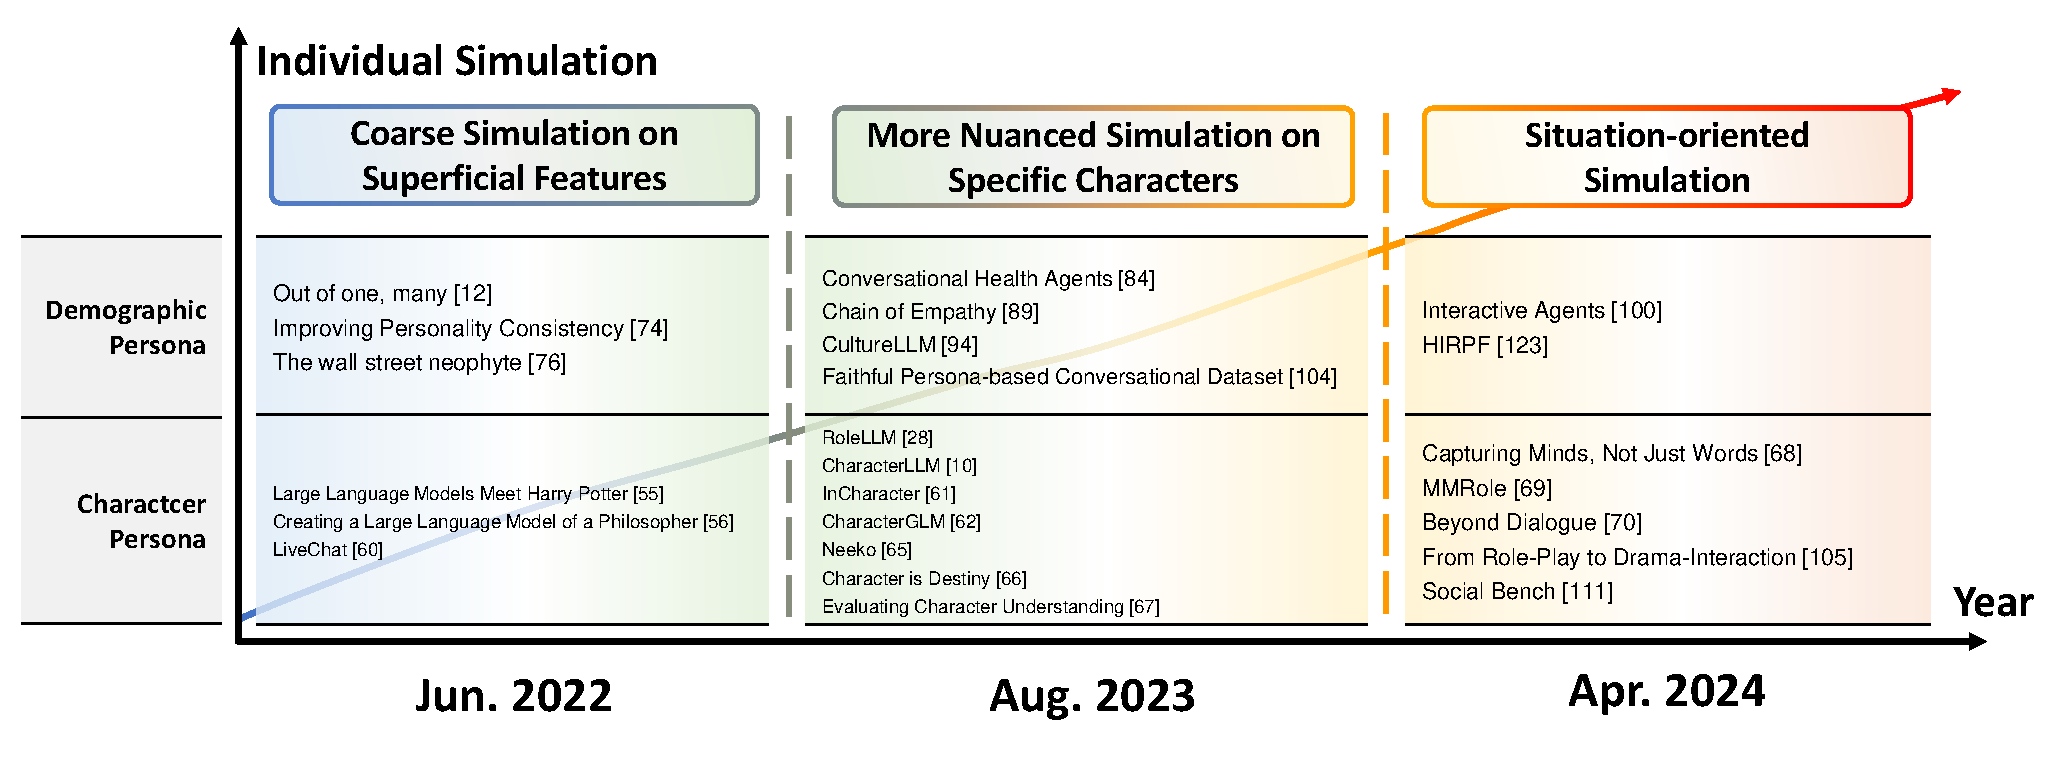
\includegraphics[width=\linewidth]{figs/trend_invi_v4.pdf}
    \caption{Illustration of individual simulation trend, which goes through {\ul coarse simulation}, {\ul more nuanced simulation}, and {\ul situation-oriented simulation}.}
    \label{fig:indi_trend}
\end{figure*}

\begin{figure*}[t]
    % \setlength{\abovecaptionskip}{-1cm}
    \centering
    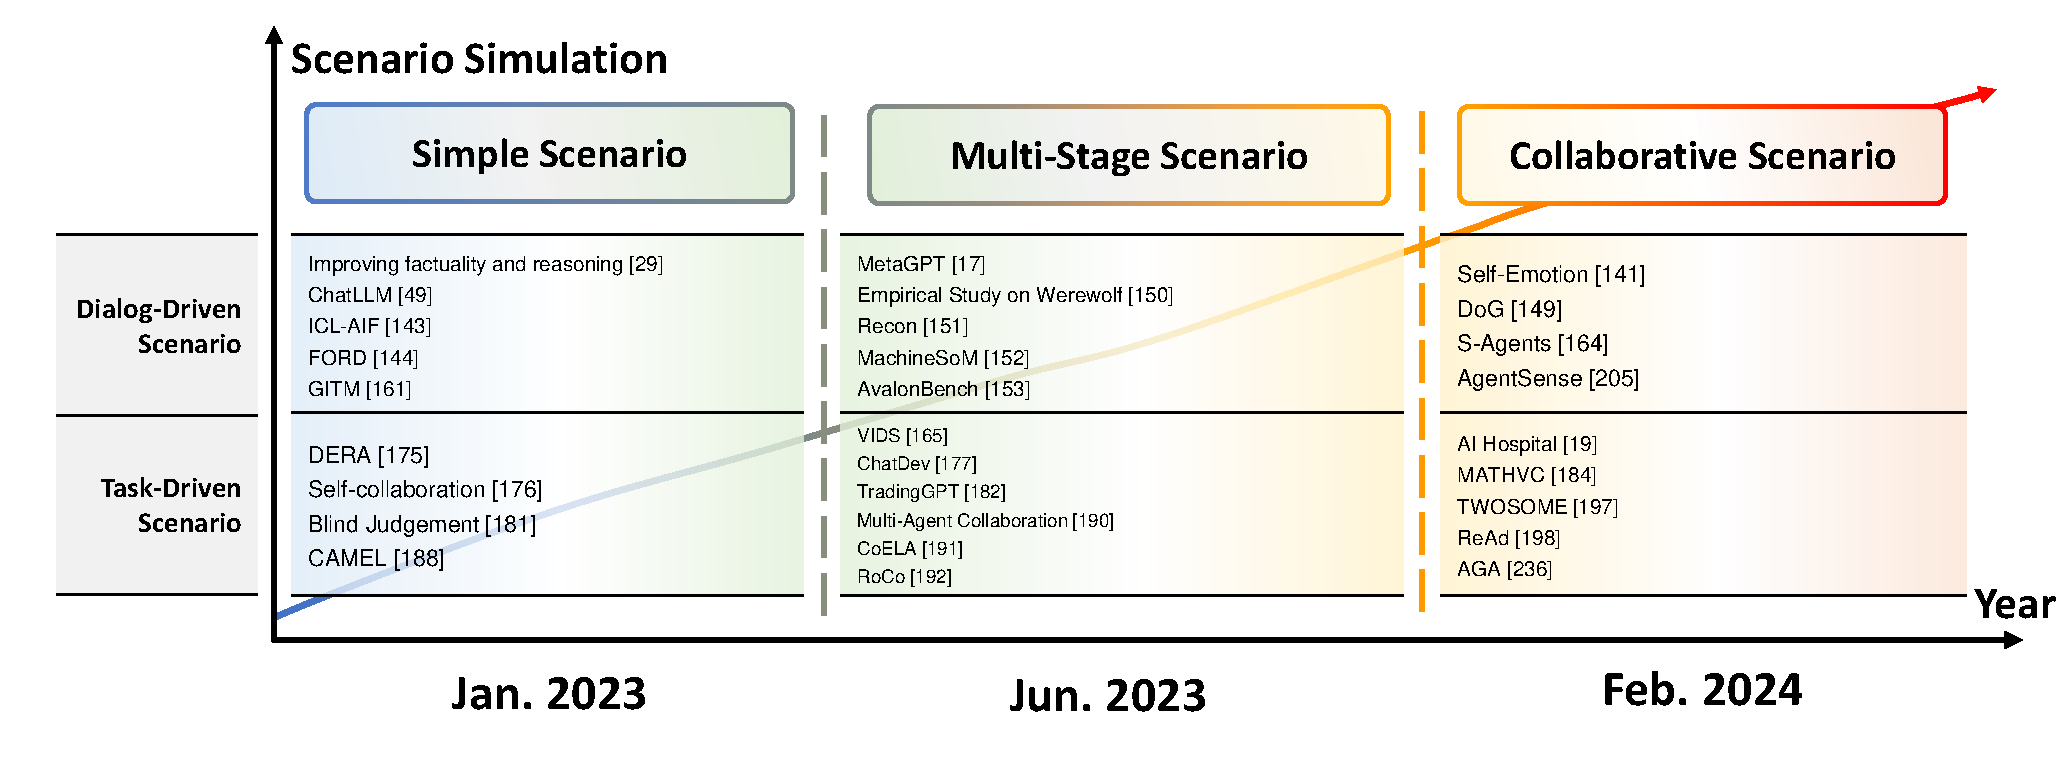
\includegraphics[trim=8mm 0mm 0mm 0mm, width=\linewidth]{figs/trend-task_v3.pdf}
    \caption{Illustration of scenario simulation trend, which goes through {\ul simple scenario}, {\ul multi-stage scenario}, and {\ul collaborative scenario}.}
    \label{fig:task_trend}
\end{figure*}

\begin{figure*}[t]
    \centering
    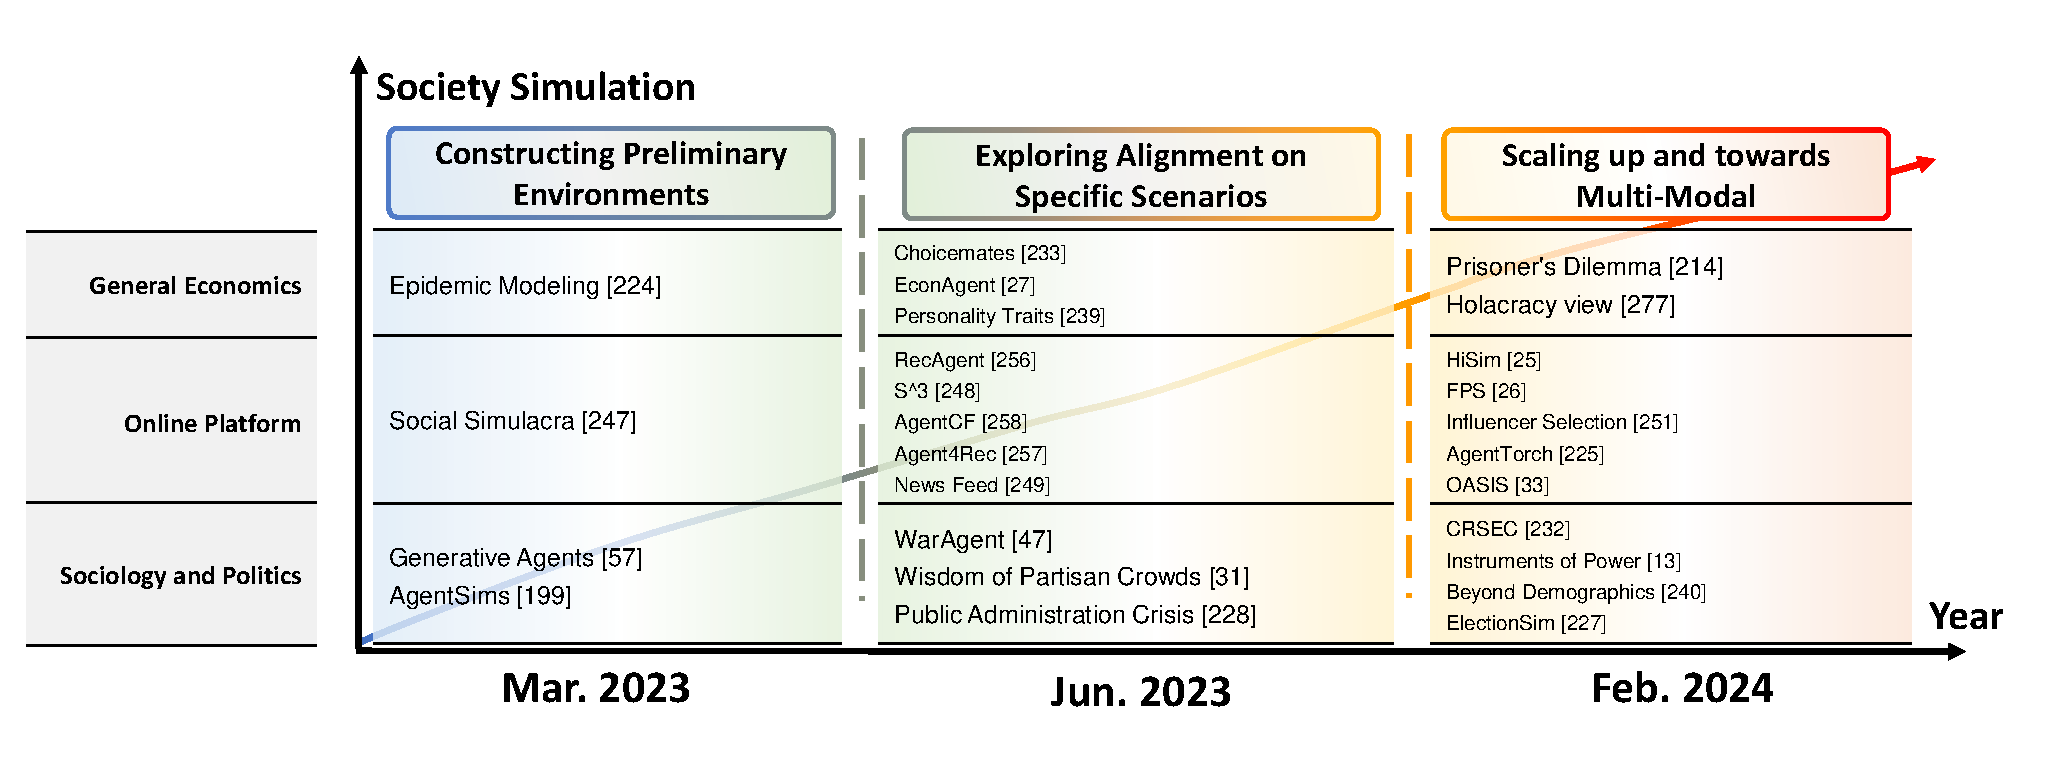
\includegraphics[width=\linewidth]{figs/trend-soc_v3.pdf}
    \caption{Illustration of society simulation trend, which goes through three stages: {\ul constructing preliminary environments}, {\ul exploring alignment on specific scenarios}, and {\ul scaling up} while moving {\ul towards multi-modal}.}
    \label{fig:soc_trend}
\end{figure*}

Evolving from social science, individual simulation powered by LLMs has progressed through three distinct stages, namely \textbf{coarse simulation}, \textbf{more nuanced simulation}, and \textbf{situation-oriented simulation}, which is depicted in Figure~\ref{fig:indi_trend}. Since \textit{{\ul June 2022}}, researchers started to focus on coarse simulations, especially for superficial traits like testing the personalities of LLMs and simulating well-known characters~\cite{serapiogarcía2023personalitytraitslargelanguage,liu2023agentbenchevaluatingllmsagents}. After \textit{{\ul August 2023}}, the trends shifted towards more refined simulations of specific individuals, with studies evaluating the cognitive aspects of simulated models~\cite{wang2024incharacterevaluatingpersonalityfidelity,yuan2024evaluatingcharacterunderstandinglarge} and improving their simulation capabilities~\cite{abbasian2024conversationalhealthagentspersonalized,yu2024neekoleveragingdynamiclora}. By \textit{{\ul May 2024}}, researchers began conducting individual simulations in specific scenarios~\cite{chen2024socialbenchsocialityevaluationroleplaying,yu2024dialogueprofiledialoguealignmentframework}, further expanding the complexity and realism of these simulations.

\subsubsection{Coarse Simulation on Superficial Features}
Many individual simulation works born since June 2022, the majority of which initially focus on simulating superficial features implied in human behaviors. A significant portion of the effort was dedicated to collecting and standardizing character-related information to build persona-based datasets~\cite{chen2023largelanguagemodelsmeet,schwitzgebel2023creatinglargelanguagemodel}. Additionally, eliciting the underlying demographic personalities of prevailing LLMs posed a challenge in this early stage~\cite{serapiogarcía2023personalitytraitslargelanguage,pan2023llmspossesspersonalitymaking}. The early trials on coarse individual simulations shed light on LLMs' attributes during simulation, including hallucinations, inherent biases, and stereotypes, which are proven to be crucial for future simulations.


\subsubsection{More Nuanced Simulation on Specific Characters}
As individual simulation methods advanced, the precision of simulations significantly improved. 
More nuanced aspects of the individual simulation gained growing attention. Some works implement new functionalities and refine the models' architecture, such as incorporating memory and planning modules~\cite{abbasian2024conversationalhealthagentspersonalized,xu2024characterdestinylargelanguage}, while others focus on designing specific tasks for training and evaluation, like multi-dimensional interviews~\cite{wang2024incharacterevaluatingpersonalityfidelity} and simulation with rich information from scene descriptions and experiential memories~\cite{wang2024rolellmbenchmarkingelicitingenhancing}.

% One approach to enhancing the simulation capabilities of LLMs involved implementing new functionalities and refining the models' architecture, such as incorporating memory and planning modules~\cite{abbasian2024conversationalhealthagentspersonalized,xu2024characterdestinylargelanguage}. Another improvement strategy focused on modifying the training processes and evaluation methods. Researchers designed specific tasks for training and evaluation, like multi-dimensional interviews~\cite{wang2024incharacterevaluatingpersonalityfidelity}, and provided LLMs with more detailed information, such as scene descriptions and experiential memories~\cite{wang2024rolellmbenchmarkingelicitingenhancing}.

\subsubsection{Situation-Oriented Simulation}
Situation-oriented individual simulations begin within game environments~\cite{light2023avalonbenchevaluatingllmsplaying}, where LLMs are required to make appropriate decisions based on predefined rules. In more complex environments, simulated individuals are supposed to interact dynamically with their surroundings, responding to real-time environmental feedback~\cite{chen2024socialbenchsocialityevaluationroleplaying,qiu2024interactiveagentssimulatingcounselorclient}. Beyond traditional simulations like dialogue, situation-oriented simulations expand into areas such as dramatic performances~\cite{wu2024roleplaydramainteractionllmsolution}, digital game exploration~\cite{wang2023voyageropenendedembodiedagent}, and 3D task execution~\cite{huang2024embodiedgeneralistagent3d}. As the complexity of these simulations grows, the demands on the underlying architecture grow as well.
% Multimodal models are employed to fulfill the need to incorporate vision modules to process graphical information~\cite{yu2024dialogueprofiledialoguealignmentframework}.

% \subsubsection{Trend of Evaluation}
% The evaluation of individual simulation has evolved from single-turn evaluation to situation-based evaluation. Traditional methods for assessing individual simulations often rely on simple open-ended questions to elicit models' attributes, with human or LLM-based annotations providing subjective evaluations. In contrast, objective evaluation methods ask the simulating LLMs to make decisions or rank outputs. Some studies have introduced mathematical metrics, like ROUGE and BLUE, to quantify the quality of the generated responses. With the advent of individual simulation, situation-based evaluation has been developed to assess the specific capabilities of LLMs in more realistic, context-rich scenarios. They often combine subjective and objective methods and consider LLMs' performance in a multi-turn interaction.


\subsection{Trend of Scenario Simulation}
The development of scenario simulation has progressed through several distinct stages. 
Starting from \textit{{\ul January 2023}}, different researches focused primarily on simple scenarios concerning single objectives and facilitated basic contextual interactions~\cite{nair2023dera,li2023camel,hamilton2023blind,xiong2023examining}.
By \textit{{\ul June 2023}}, the emphasis changed to multi-stage scenarios, incorporating multi-step tasks that enabled agents to engage in sequential decision-making and adaptive responses across varied contexts to achieve the more complex goal~\cite{talebirad2023multi,mandi2024roco,li2023tradinggpt,hassan2023chatgpt}.
By \textit{{\ul February 2024}}, research has increasingly focused on multi-agent collaborative scenarios, emphasizing agents' capabilities to cooperate and adapt within complex, high-order simulations~\cite{yu2024affordable,chen2024s,ma2024debate,yue2024mathvc}.

\subsubsection{Simple Scenario}
In the initial phase of scenario simulation, researchers focused on constructing simple scenarios that supported foundational agent interactions. Much of this work concentrated on dialogue-driven decision-making frameworks, which facilitated structured information exchange and agent alignment~\cite{nair2023dera,li2023camel,hao2023chatllm}. Additionally, studies explored the collaborative potentials of agents through multi-agent debate frameworks, employing debate and critical feedback to assess cooperative reasoning and performance enhancement in LLMs~\cite{fu2023improving,xiong2023examining,du2023improving}. Simultaneously, other studies applied scenario simulations within specific domains—such as law, software development, scientific analysis, and recommendation systems—demonstrating the versatility of task-based simulations in achieving domain-specific objectives~\cite{hamilton2023blind,dong2023self,zhu2023ghost}.

\subsubsection{Multi-Stage Scenario}
Different from simple task-oriented scenarios, multi-stage scenarios are no longer limited to mere agent interactions. Instead, they emphasize the fine-grained construction of scenarios. 
This stage introduces multiple roles and task decomposition as central elements, enabling agents to collaborate not merely on single tasks but through incremental task breakdowns that require coordinated effort~\cite{zhang2023building,mandi2024roco}. 
In software development, ~\cite{qian2024chatdev,hong2023metagpt} decomposed the development process into multiple stages like design, coding and testing to enhance the capacity for achieving complex objectives and improving software quality.
Additionally, communication games were introduced to investigate human behavior within complex conversational scenarios, adding depth to interaction analysis~\cite{xu2023exploring,wang2023avalon,zhang2023exploring,light2023text}.

\subsubsection{Collaborative Scenario}
With the growing interest in scenario simulation, research shifted toward collaborative scenarios, emphasizing advanced social dynamics and cooperative strategies in agent interactions. \cite{tan2024true,zhang2024towards} introduce reinforcement learning to align LLM with embodied environments. 
To build efficient scenario simulations, \cite{yu2024affordable} focused on reducing LLM inference costs by modeling social relationships while \cite{chen2024s} utilized dynamic ``agent trees'' in environments like Minecraft, enabling asynchronous task execution for efficient resource gathering. 
In addition, \cite{fan2024ai,yan2024social} simulated collaborative environments in the real world, reflecting complex social interactions such as medical processes and the development of social skills, with agents handling evolving multistep tasks.




\subsection{Trend of Society Simulation}
Since the concept of social simulation was first introduced by Park et al. \cite{park2022social}, numerous notable studies have emerged. Broadly, the development of this field can be categorized into three phases. Prior to \textit{{\ul June 2023}}, researchers concentrated on constructing preliminary environments \cite{park2023generative,williams2023epidemic,lin2023agentsims}. By \textit{{\ul February 2024}}, the focus shifted toward exploring alignment within specific scenarios, such as persona modeling and targeted environments, marking the first significant surge of publications \cite{gao2023s3,wang2023avalons,li2024econagent}. Most recently, the trend has moved towards scaling up and incorporating multi-modal approaches. In this phase, large-scale precise modeling has gained recognition, with other modalities such as vision and voice being integrated into simulations \cite{mou2024unveiling,ren2024emergence,wu2024enhance,wang2024grutopia}.

The main characteristics can be summarized as:
\subsubsection{Constructing Preliminary Environments}
The complexity of society simulation, to a certain extent, stems from the complexity of the environment involved. Society simulation usually involve multiple interacting individuals (such as people, organizations, groups, etc.), which act in a specific environment (such as cities, markets, cyberspace, etc.). Therefore, the pioneer work focuses on how to design a specific environment to support society simulation. \cite{park2023generative} built an interactive sandbox environment by extending a LLM to store a complete record of an agent's experience and dynamically synthesizing memory to plan behavior. \cite{williams2023epidemic} built an epidemic spread simulation environment that simulates human behavior at the individual level to reproduce the spread of an epidemic in a simulated environment. \cite{lin2023agentsims} created an easy-to-use infrastructure that allows researchers to build evaluation tasks by adding agents and buildings, providing a visual and program-based platform for testing LLMs.

\subsubsection{Exploring Alignment on Specific Scenarios}
With the development of simulation environment technology, society simulation has basically become operational. At this time, to test the credibility of simulation, evaluating the alignment performance of agents with real situations on specific tasks has gradually become an important research direction. \cite{gao2023s3} use real social network data to measure the accuracy of simulation by evaluating the behavior and decision-making of agents at the individual and group levels in a simulated social network environment. \cite{li2024econagent} evaluate the decision rationality of LLM agents by simulating macroeconomic activities and comparing the performance of LLM agents with traditional rule-based agents or language agents in generating classic macroeconomic phenomena such as inflation and unemployment.

\subsubsection{Scaling Up and towards Multi-Modal}
\paragraph{Scaling up} Before LLM-based agents became widely adopted for society simulation, researchers predominantly relied on agent-based modeling (ABM) methods, where agents were typically programmed to react based on predefined algorithms. With the advent of LLM providing glimpses of human-like intelligence \cite{browning2023personhood}, LLM-based agents entered the spotlight. Given the good performance of LLM-based agents in a series of specific scenarios, researchers began to expand the scale of simulation. \cite{mou2024unveiling, ren2024emergence} involve the core elements of large-scale society simulation and study the interaction between agents and the generation of behavioral norms. \cite{wu2024enhance} proposed a proving ground for assessing advanced reasoning capabilities of LLM agents in a large-scale society simulation context.
% Initially, due to the high computational costs of each prompt, simulations typically included fewer than five LLM agents, often accompanied by several ABM agents. However, as computational efficiency improved, simulating over 100 agents became feasible. Naturally, the more agents involved, the more human-like the simulation tends to be.
% \cite{conte2012manifesto} mentioned that real-world societies imply several levels of complexity, which are not reduced to the micro and the macro levels but include intermediate levels (groups, tribes, networks, communities, etc.).
% According to the scale of agents,there can be categorized generally three scales of such simulations: fewer than ten agents can be referred to as a "club", eleven to 100 agents can be considered a "party", and simulations with more than 100 agents can be classified as a "society".

\paragraph{Multi-Modal} With the development of language models, using language agents for society simulation has become a hot topic in research. It incorporates other modal information elements such as vision in life into the simulation through text descriptions. However, with a series of advances in the field of Vision-Language Model(VLM)~\cite{Radford2021, liu2024visual, achiam2023gpt}, researchers began to incorporate VLM-based agents into society simulation research. \cite{wang2024grutopia} provide rich multi-modal interaction information and detailed annotations in large-scale scenarios. \cite{yu2024mineland} focus on simulating the perceptual limitations and physical demands of the real world to facilitate more realistic social interactions.
% Since 2021, the OpenAI team introduced CLIP\cite{Radford2021}, marking the advent of multi-modal LLMs. Vision-language models like LLaVA\cite{Liu2024} and GPT-4\cite{achiam2023gpt} significantly enhance agents' perceptual capabilities, enabling them to sense the real world or engage in sandbox games\cite{wang2024grutopia，Gong2023}. Recent studies also highlight the incorporation of sound as a factor\cite{Yu2024，wu2024enhance}. 

% As embodied AI continues to evolve, it is reasonable to predict that LLM agents will increasingly serve as core administrative components, incorporating additional modalities such as touch and taste in the near future.

% \subsubsection{Precise Persona}
% %The concept of persona modeling in LLM-based agents for social simulations gained significant attention around 2023. Early contributions, such as Chateval\cite{chan2023chateval}, introduced the use of predefined personas to evaluate LLM agents within simulated environments, emphasizing the agents' interactions with their surroundings and their responses based on assigned personas. This approach established structured tasks for assessing agents' social behavior, positioning persona modeling as a crucial component in social simulation research.

% %The Names-dataset\cite{NameDataset2021}, a widely used persona library, offers a diverse collection of names categorized by gender and ethnicity, facilitating research in natural language processing and machine learning. In addition to publicly available resources, many researchers employ self-collected datasets, either sourced online or generated using AI. Recent advancements, such as PersonaGym\cite{Samuel2024}, further contribute by providing a dynamic evaluation framework and metrics tailored for persona agents in LLMs.

% The modeling of precise personas in LLM-based agents has become a key research area in social simulation, especially since 2023. Early works, such as Chateval \cite{chan2023chateval}, introduced the use of predefined personas to evaluate agents' interactions with their environments, highlighting the importance of persona consistency in social behavior simulations. This approach has led to the development of structured tasks for assessing agents' social behavior, marking persona modeling as an essential component of social simulation research.

% Several resources support persona modeling, such as the Names-dataset \cite{NameDataset2021}, which offers a diverse array of names categorized by gender and ethnicity, facilitating research in natural language processing and machine learning. Researchers also use self-collected datasets sourced online or generated by AI tools. Recent developments, such as PersonaGym \cite{Samuel2024}, have further contributed by providing dynamic frameworks and evaluation metrics tailored to persona agents in LLM-based social simulations.

% At the same time, social simulations can be classified into macro-level and micro-level approaches \cite{gao2023s3}. Early research predominantly focused on macro simulations of societal systems, such as the study of epidemics or economic systems \cite{williams2023epidemic，Zhang2024on，hua2023war，li2024econagent}. Macro simulations aim to model the large-scale dynamics of society, often at the expense of detailed individual characterization, whereas micro simulations focus on the behavior of smaller groups, revealing more intricate social actions like collaboration, competition, or negotiation \cite{chen2023agentverse，xu2023exploring，han2023guinea，jarrett2023language}.

% With the introduction of LLM-based agents, micro-level simulations have gained prominence, allowing researchers to observe emergent behaviors at a granular level. However, micro simulations can sometimes lack the broader context provided by macro-level approaches. Recent works have begun to combine both scales—macro and micro—to improve simulation accuracy and efficiency. For instance, agent-based models (ABMs) have been used to simulate the behaviors of individuals while considering larger social structures, thus offering a more nuanced perspective on societal dynamics \cite{mou2024unveiling，zhao2024hierarchical，xiao2023simulating}. In addition, some studies explore both perspectives simultaneously, analyzing phenomena through the lens of both micro and macro scales \cite{zhaocompeteai}.

% Ultimately, the integration of macro and micro simulations is essential for creating a comprehensive and realistic model of entire societies. By combining both levels of analysis, we can achieve a more accurate and effective representation of the complex dynamics that govern social systems.

% \subsubsection{Multi Modal}
% LLMs primarily operate within a text modality, simulating human language usage, while most social simulation research has relied on pure LLMs. Since 2021, the OpenAI team introduced CLIP\cite{Radford2021}, marking the advent of multi-modal LLMs. Vision-language models like LLaVA\cite{Liu2024} and GPT-4\cite{achiam2023gpt} significantly enhance agents' perceptual capabilities, enabling them to sense the real world or engage in sandbox games\cite{wang2024grutopia，Gong2023}. Recent studies also highlight the incorporation of sound as a factor\cite{Yu2024，wu2024enhance}. As embodied AI continues to evolve, it is reasonable to predict that LLM agents will increasingly serve as core administrative components, incorporating additional modalities such as touch and taste in the near future.

%\subsubsection{Macro Micro}
%\XY{``Macro Micro” does not sound like a term, and this section doesn’t clarify whether the focus is more on the macro or micro level. It seems like it should be discussed alongside ``more precise persona.”}
%Social simulation can be categorized into macro-level and micro-level simulations \cite{gao2023s3}. Early works predominantly focused on macro simulations of societal scenarios \cite{williams2023epidemic}\cite{Zhang2024on}\cite{hua2023war}\cite{li2024econagent}. Macro simulation emphasizes the overall dynamics of societal systems, often at the expense of precise characterization of individuals, which contrasts with micro simulation. Concurrently, theoretical topics such as game theory and social science interpretations can also be classified into macro and micro simulations based on the scale of experimental validation \cite{suzuki2024evolutionary}\cite{Zhu2024}.

%With the advancement of LLM-based agents, micro-level simulation has gained prominence recently\cite{lin2023agentsims}. By observing small groups of individuals, researchers are uncovering hidden social actions, including emergent collaboration, betrayal, competition, and negotiation\cite{chen2023agentverse}\cite{xu2023exploring}\cite{han2023guinea}\cite{jarrett2023language}. Some recent studies have attempted to integrate macro and micro approaches to enhance efficiency; for instance, employing agent-based modeling (ABM) to simulate ordinary individuals while focusing on social structures to provide a more nuanced view of administrators\cite{mou2024unveiling}\cite{zhao2024hierarchical}\cite{xiao2023simulating}. At the same time, some works like\cite{zhaocompeteai} analysis the phenomena on both micro and macro perspectives.

%Ultimately, macro simulations can lack precision and realism, while micro simulations may overlook the broader context. Therefore, it is reasonable to assert that only by combining macro and micro simulations can we truly achieve the goal of accurately simulating entire societies.
